\graphicspath{{chapters/c5_transient_binding/si-figures/}}
%============================ MAIN ==========================
\section{Supporting Info}
\begin{figure}[ht]
  \centering
  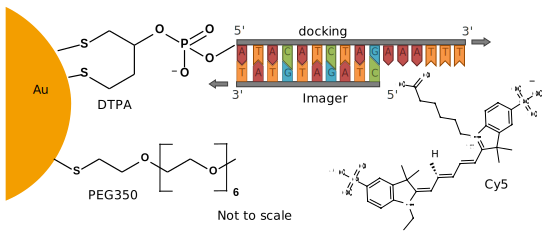
\includegraphics[width=0.8\textwidth]{AuNR-SS_bonding}
  \makeatletter
  \renewcommand{\fnum@figure}{\figurename~S\thefigure}
  \makeatother
  \caption{\textbf{Binding to Gold surface} The chemical structures of different components in the transient binding scheme.
  The docking strand is attached to the nanorod through DTPA which has two thiols attached to the gold atoms.
  The sequence of the docking and the imager strand are shown with their complementary binding.
  The imager strand is labeled with Cy5 at its $3\prime$ end.
  The rest of the nanorod surface is functionalized with PEG350 which has 9 monomers giving it a length of \SI{\sim3}{\nm}.}
  \label{SIfig:AuNR-SS_bonding}
\end{figure}

\begin{figure}[ht]
  \centering
  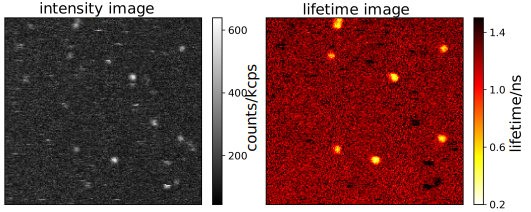
\includegraphics[width=0.8\textwidth]{trans_int_lt_img}
  \makeatletter
  \renewcommand{\fnum@figure}{\figurename~S\thefigure}
  \makeatother
  \caption{A \SI[product-units=power]{10x10}{\um} scanning image of the surface of the substrate with gold nanorod functionalized with docking strand and mPEG7-SH.
  The solution contains \SI{100}{\nM} imager strand in PBS pH 7.4 buffer with \SI{500}{\mM} \ce{NaCl}.
  The image on the left shows counts per millisecond while the image on the right shows the lifetime.
  The brgiht spots on the lifetime image corresponds to the gold nanorod as they have much shorter life time than the IRF.}
  \label{SIfig:trans_int_lt}
\end{figure}
% \subsection*{Replenish and recyacle}
\begin{figure}[ht]
  \centering
  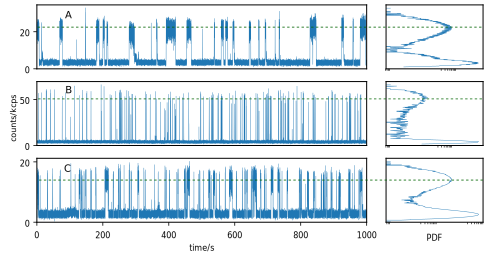
\includegraphics[width=\textwidth]{bleaching_free_longtrace}
  \makeatletter
  \renewcommand{\fnum@figure}{\figurename~S\thefigure}
  \makeatother
  \caption{\textbf{Many single-molecule per nanorod.} Time traces of three different nanorods with a single binding sites each but different enhancement factors.
  The histogram of intensity for each time trace is shown in the right and the two peaks indicates the presence of only one observable docking strand.
  Notice the different binding kinetics of trace-A and trace-B though they have similar enhancement factor.}
  \label{SIfig:bleaching_free_longtrace}
\end{figure}

\begin{figure}[ht]
  \centering
  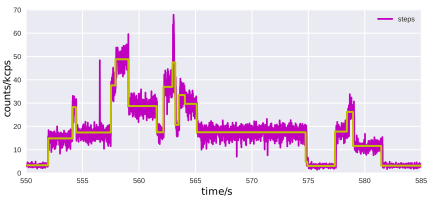
\includegraphics[width=0.8\textwidth]{step_timetrace}
  \makeatletter
  \renewcommand{\fnum@figure}{\figurename~S\thefigure}
  \makeatother
  \caption{Time trace on a functionalized gold nanorod with multiple transient binding appearing on top of each other.
  The association and dissociation of each imager strand can be distinguished from the step hight and the time of appearance. }
  \label{SIfig: step_transbind}
\end{figure}
% \subsection*{Transient binding on substrate}
\begin{figure}[ht]
  \centering
  \includegraphics[width=0.8\textwidth]{timetrace_only_Cy5}
  \makeatletter
  \renewcommand{\fnum@figure}{\figurename~S\thefigure}
  \makeatother
  \caption{\textbf{Transient binding without nanorod:} (A) The shematic of the transient binding.
  Docking strand was immobilized on the surface through neutravidin and biotin bonding.
  The solution contained \SI{100}{\nM} imager-Cy5 in PBS pH 7.4 buffer.
  Scanning image  in the absense (B) and presence (C) of docking strand on the surface showing the specificity of binding of the imager to the docking strand.
  (D) Time trace of transient binding on a single neutravidin-docking site at \SI{\sim 0.1}{\kW\per\cm\squared} power density, 10 times higher than the laser power used for measurement on the nanorod. The burst heights are \SI{\sim 20}{ kcps} corresponding to single imager-Cy5.
  To compare with the bursts from nanorods and calculate enhancement factor, the count rate can be devided by 10 to match the laser power on the nanorod as the intensity varies linearly at such lower range of powers.
  A count rate of \SI{2}{ kcps} for unenhanced Cy5 will be used in the main text. 
  }
  \label{SIfig:timetrace_only_Cy5}
\end{figure}
% \subsection*{Dissociation of docking strand}
\begin{figure}[ht]
  \centering
  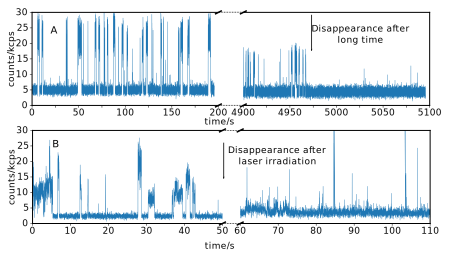
\includegraphics[width=\textwidth]{dissociation_transbind}
  \makeatletter
  \renewcommand{\fnum@figure}{\figurename~S\thefigure}
  \makeatother
  \caption{\textbf{Dissociation of docking strand.}
  (A) The time trace on the top is recorded on a gold nanorod as long as the docking strand on it disappears.
  The transient binding never appeared again even after re-flushing with imager strand and realigning then laser focus.
  (B) The transient binding trace on a gold nanrod before and after irradiation with high laser power (\SI[per-mode=repeated-symbol]{1000}{\watt\per\cm\squared}, \SI{40}{\MHz}).
  }
  \label{SIfig:dissociation_transbind}
\end{figure}